
\chapter{毛国瑶抄录靖藏本批语}

所谓靖藏本,因原为扬州靖应鵾所藏而得名。此书一九五九年夏由毛国瑶发现,一九六四年尚在,后迷失不知下落。据介绍原书题``石头记''。存七十八回。缺第二十八与二十九回,第三十回残失三页。

书发现时,毛国瑶曾将书中批语与戚本进行比较,摘录戚本所无的批语一百五十条,过录在横行练习簿上。后来将它发表于南京师范学院《文教资料简报》一九七四年八、九月号(总第二十一、二十二合刊)。

此本中独有一些极重要的批语。如第十三回命作者删去``秦可卿淫丧天香楼''、``遗簪、更衣诸文''的人是畸笏叟;如第二十二回畸笏叟所加的批语``前批知者聊聊,不数年,芹溪、脂砚、杏斋诸子皆相继别去。今丁亥,只馀朽物一枚,宁不痛杀!''都极有研究资料价值。此外,批语中还提供了许多先前不知道的八十回后的佚稿情节。

由于靖本只有毛国瑶一人亲见过,近年有不少研究者怀疑此本并不存在。详细情况可参阅裴世安老先生编辑的《靖本资料》(自印本,2005年)。

第一回

1.作者自己形容{(\kaishu ``生得骨格不凡,丰神迥异''句墨笔眉批)}

2.补天济时勿认真作常言{(\kaishu 女娲炼石补天一段侧批)}

3.佛法亦须赏还况世人之债乎游戏笔墨{(\kaishu ``待劫终之日复还本质''
句侧批)}

4.赖债者来看此句{(\kaishu 同3侧批)}

5.果有奇贵自己亦不知若以奇贵而居即无真奇贵{(\kaishu ``不知赐了弟子那几段奇处''句墨眉)}

6.事则实事然亦得叙有曲折有隐现有带架有逆间有正辟空谷以至草蛇灰线传声一击两鸣明修栈道暗度陈仓两山雾雨云龙对峙托月烘云背面传粉万染千皱诸奇秘法亦复不少予亦逐回搜剔刹破明白以待高明批示开卷一篇立意真打破历来小说果臼阅其笔则是庄子离骚之亚{(\kaishu ``按迹寻踪''句墨眉)}

7.这是画家烟云模糊处不被蒙敝方是巨眼{(\kaishu ``并题一绝云''一段墨眉)}

8.无是儿女之情始有夫人之分{(\kaishu ``也就丢过不在心上''句侧批)}

9.走罢二字如见如闻非过来人若个能行{(\kaishu ``士隐便说一声走罢''句墨眉)}

第二回

10.向只见集古集唐句未见集俗语者{(\kaishu ``偶因一着错便为人上人''墨眉)}

11.是智者方能通谁为智者一叹{(\kaishu ``智通寺''三字墨眉)}

12.雨村聿意还是俗眼只识得双玉等未觉之先却不晓既证之后{(\kaishu 遇龙钟老僧一段朱眉)}

第三回

13.君子可欺以其方也雨村当王莽谦恭下士之时即政老亦为所惑作者指东说西{(\kaishu ``且贾政最喜读书之人''句墨眉)}

14.阿凤三魂已被作者勾走了后文方得活跳纸上{(\kaishu ``我来迟了不曾迎接远客''句墨眉)}

15.文字不反不见正文似此应从国策得{(\kaishu ``不知是怎生个惫懒人物懵懂顽童''墨眉)}

16.宝玉知己全用体贴工夫{(\kaishu ``倘或摔坏了那玉岂不是因我之过''侧批)}

第四回

17.四家皆为下半部伏根{(\kaishu ``这四家皆连络有亲\ldots{}''句侧批)}

18.批书亲见一篇薄命赋特出英莲{(\kaishu 叙英莲遭遇一段墨眉)}

19.无名之症即是病之名而反曰无像极{(\kaishu ``已得无名之病''句侧批)}

20.庙了结文字伏下伏又千里线胡卢字样起胡卢字样结盖一部书皆系胡提之意也知乎{(\kaishu 充发门子一段墨眉)}

国瑶按:第一册封面下粘一长方形字条,长五寸,宽约三寸半,左下方撕缺,可见``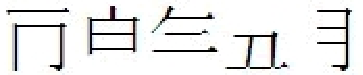
\includegraphics[width=20mm]{../images/00032}录''字样,墨笔书写,内容如下:

紫雪溟蒙楝花老蛙鸣厅事多青草庐江太守访故人浔江并驾能倾倒两家门第皆列戟中年领郡稍迟早文采风流政有馀相逢甚欲抒怀抢于时亦有不速客合坐清炎斗炎嫡岂无炙鲤与寒鷃不乏蒸梨兼蝓芫瀹枣二簋用享古则然宾酬主醉今诚少亿首宿卫明光宫楞伽山人貌狡好马曹狗监共嘲难而今触痛伤怀抱交情独剩张公子晚识施君通纻红缟多闻直谅复奚疑此乐不殊鱼在藻始觉诗书是坦途未妨车轱当行潦家家争唱饮水词纳兰小字几曾知布袍廓落任安在说向名场尔许时

第五回

21.寡母孤儿毕有真{(\kaishu ``不如你各自住着好任意施为''侧批,此条应在第四回,误抄在此)}

22.此句定评想世人目中各有所取也按黛玉宝钗二人一如姣花一如纤柳各极其妙者皆性分甘苦不同世人之故耳{(\kaishu ``人多谓黛玉所不及''句下小字夹批)}

23.八字为二玉一生文字之纲{(\kaishu ``求全之毁''句墨眉)}

24.恰极补裘回中与此合看{(\kaishu ``寿夭多因毁谤生多情公子空牵念''句墨眉)}

25.绛芝轩诸事由此而生{(\kaishu 朱眉)}多大胆量敢作此文{(\kaishu 墨眉)(``吾所爱汝者乃天下古今第一淫人也''句批)}

26.宝玉心性只是体贴二字故为意淫{(\kaishu ``惟心会而不可口传''句侧批)}

第六回

27.宝袭亦大家常事耳已令领意淫之训{(\kaishu 回前批)}

28.借刘妪写阿凤正传非泛文可知且优二进三进巧姐归着{(\kaishu 回前批)}

29.一段云雨之事完一回提纲文字{(\kaishu 宝玉袭人一段侧批)}

30.能两亩薄田度日方说的出{(\kaishu ``守多大碗儿吃多大碗的饭''句墨眉)}

31.骂死世人可叹可悲{(\kaishu ``我又没有收税的亲戚''一段墨眉)}

32.要紧人虽未见有名想亦在副册内者也{(\kaishu ``先找着凤姐一个心腹通房大丫头名唤平儿''句下小字夹批)}

33.观警幻情榜方知余言不谬{(\kaishu 同上句朱眉)}

34.虽平常而至奇稗官中末见{(\kaishu ``手内拿着小铜火筋儿''句墨眉)}

35.五笑写凤姐活跃纸上{(\kaishu 与刘姥姥对话墨眉)}

36.何如当知前批不谬{(\kaishu 同上句墨眉)}

37.穷亲戚来是好意思余又自石头记中见了叹叹数语令我欲哭{(\kaishu ``瞧瞧我们是他的好意思''
句墨眉)}

38.也是石头记见了叹叹{(\kaishu ``怎好教你空手回去呢''句墨眉)}

39.如见如闻此种话头作者从何想来应是心花欲开之侯{(\kaishu 凤姐与刘姥姥对话一节墨眉)}

40.引阿凤正文借刘妪入初聚金玉为写送宫花真变幻难测读此等文字非细究再三再四不计数不能领会叹叹{(\kaishu 回后批,墨笔)}

第七回

41.他小说中一笔作两三笔者一事启两事者均曾见之岂有似送花一回间三带四赞花簇锦之文哉{(\kaishu 回前批)}

42.作出鲸卿随笔却闲闲先妯娌一聚带出一丝不见造{(\kaishu 秦氏凤姐说话一段墨眉)}

43.焦大之醉伏可卿死作者秉刀斧之笔一字一泪一泪化一血珠惟批书者知之{(\kaishu 焦大醉骂一节墨眉)}

第八回

44.本意正传是实曩时苦恼叹叹{(\kaishu ``再或可巧遇见他父亲''句朱眉)}

45.沾光善骗人无星戥皆随事生情调侃世人余亦受过此骗阅此一笑三十年前作此语之人观其形已皓首驼腰矣使彼亦细听此语彼则潸然泣下余亦为之败兴{(\kaishu ``多早晚赏我们几张贴贴''句墨眉)}

46.十六字乃宝卿正传参看前写黛玉传各不相犯令人左右难其于毫末{(\kaishu ``罕言寡语''四句墨眉)}

47.试问此一托比在青埂下啼啸声何如{(\kaishu ``宝钗托于掌上''句朱眉)}

48.余代答云遂心如意{(\kaishu 同上句墨眉)}

49.伏下文又夹入宝钗不是虚图对的工{(\kaishu ``好知运败金无彩''句墨眉)}

50.前回中总用灰线草蛇细细写法至此方写出是大关节处奇之至{(\kaishu 宝钗看玉一段墨眉)}

51.可知余前批不谬{(\kaishu 墨眉)}

52.别人者袭晴之辈也{(\kaishu 墨眉)}

53.作者抚今之事尚记今金魁星乎思昔肠断心催{(\kaishu 墨眉)}

第九回

54.此岂是宝玉所乐为者然不入家塾则何能有后回试才结社文字作者从不作安逸苟且文字于此可见{(\kaishu 入家塾一段墨眉)}

55.此以俗眼读石头记也作者之意又岂是俗人所能知余谓石头记不得与俗人读{(\kaishu 上批隔一行墨眉)}

56.安分守己也不是宝玉了{(\kaishu ``宝玉终是不能安分守己的人''墨眉)}

57.前有幻境遇可卿今又出学中小儿淫浪之态后文更放笔写贾瑞正照看书人细心体贴方许你看{(\kaishu 墨眉)}

58.声口如闻{(\kaishu ``好囚攮的们,这不都动了手了么''句墨眉)}

第十回

59.这个理怕不能评{(\kaishu ``叫他评评这个理''句侧批)}

60.吾为趋炎附势仰人鼻息者一叹{(\kaishu ``早吓的都丢在爪洼国去了''句墨眉)}

61.不知心中作何想{(\kaishu 墨眉)}

第十一回无批

第十二回

62.千万勿作正面看为幸畸笏老人{(\kaishu 贾瑞与凤姐对话一节墨眉)}

63.可为偷情者一戒{(\kaishu ``一夜几乎不曾冻死''句墨眉)}

64.教训最严奈其心何一叹{(\kaishu ``那代儒素日教训最严''句墨眉)}

65.处处点出父母痴心子孙不肖此书纯系自愧而成{(\kaishu 墨眉)}

66.调戏尚有故乎{(\kaishu ``说你无故调戏他''句墨眉)}

67.此节可入西厢内记十大快批评中畸笏{(\kaishu 凤姐泼粪一段墨眉)}

第十三回

68.此回可卿梦阿凤作者大有深意惜已为末世奈何奈何贾珍奢淫岂能逆父哉特因敬老不管然后恣意足为世家之戒秦可卿淫丧天香楼作者用史笔也老朽因有魂托凤姐贾家后事二件岂是安富尊荣坐享人能想得到者其言其意令人悲切感服姑赦之因命芹溪删去遗簪更衣诸文是以此回只十页删去天香楼一节少去四五页也一步行来错回头已百年请观风月鉴多少泣黄泉{(\kaishu 回前长批)}

69.九个字写尽天香楼事是不写之写常村{(\kaishu ``无不纳闷都有些疑心''句下小字夹批)}

70.可从此批通回将可卿如何死故隐去是余大发慈悲也叹叹壬午季春畸笏叟{(\kaishu 同上句朱眉)}

71.删却是未删之文{(\kaishu 商议料理丧事及贾珍痛哭一段朱批)}

72.何必定用西字读之令人酸笔{(\kaishu 设坛于西帆楼上一段朱眉)}

73.是亦未删之文{(\kaishu 瑞珠触柱一段朱眉)}

74.刺心之笔{(\kaishu 贾珍蹲身跪下道乏朱眉)}

75.读五件事未完余不禁失声大哭卅年前作书人在何处耶{(\kaishu ``因想头一件\ldots{}''一段朱眉)}

76.旧族后辈受此五病者颇多余家更甚卅年间事见知于卅年后令余悲痛血泪盈面{(\kaishu 同上墨眉)}

第十四回

77.用彩明因自身识字不多且彩明系未冠之童故也{(\kaishu 命彩明钉造簿册一节墨眉)}

78.数字道尽声势壬午春畸笏{(\kaishu ``浩浩荡荡''句墨眉)}

79.忙中闲笔□□玉兄作者良苦壬午春畸笏{(\kaishu ``那一位是衔宝而诞者''句墨眉。二字蛀去)}

80.牛丑清水柳乃卯也彪折虎字寅也陈即辰翼大为蛇寓巳字马午也魁即鬼鬼金羊寓未字侯申也晓鸣鸡也寓酉字豕即石亥字寓焉守业犬也所谓十二支寓焉{(\kaishu 回后批,墨笔)}

第十五回

81.伤心笔{(\kaishu ``面若春花,目似点漆''句朱眉)}

82.又写秦钟智能事尼庵之事如此壬午季春畸笏{(\kaishu 秦、智二人偷情一段墨眉)}

第十八回

83.孙策以天下为三分众才一旅项籍用江东之子弟人惟八千遂乃分裂山河宰割天下岂有百万义师一朝卷申芟夷斩伐如草木焉江淮无涯岸之阻亭壁无藩篱之固头会箕敛者合从缔交锄耰棘矜者因利乘便将非江表王气终于三百年乎是知洴吞六合不免轵道之灾混一车书无救平阳之祸呜呼山岳崩颓既履危亡之运春秋迭代不免去故之悲天意人事可以凄沧伤心者矣 大族之败必不致如此之速特以子孙不肖招接匪类不知创业之艰难当知瞬息荣华暂时欢乐无异于烈火烹油鲜花着锦岂得久乎戊子孟夏读虞子山文集因将数语系此后世子孙其毋慢忽之{(\kaishu 书眉墨笔书写,误字均未改)}

84.妙玉世外人也笔笔带写故妙极妥极畸笏{(\kaishu 墨眉)}

85.前须十二钗总未的确皆是慢终也至来回警幻榜始知情正副又副乃三四副芳讳壬午季春{(\kaishu 墨眉)}

第十九至第二十一回无批

第二十二回

86.将薛林作甄玉贾玉看则不失书执笔本旨矣丁亥夏畸笏叟{(\kaishu 墨眉)}

87.凤姐点戏脂砚执笔事今知者聊聊矣不怨夫(朱眉)前批知者聊聊不数年芹溪脂砚杏斋诸子皆相继别去今丁亥夏只剩朽物一枚宁不痛杀{(\kaishu 前批稍后墨笔)}

88.此回未补成而芹逝矣叹叹丁亥夏畸叟{(\kaishu 墨眉)}

第二十三回

89.多大力量写此一句余亦骇警况宝玉手回思十二三时亦会有是想时不再至不禁泪下{(\kaishu 贾政呼唤宝玉一段墨眉)}

90.批至此几令人失声{(\kaishu 想起贾珠一段墨眉)}

91.丁亥春日偶识一浙省客余意甚合真神品白描美人物所缘彼无暇宦缘奈不能留都下久且来几南行矣至今耳火又余帐然之至阿颦墨缘之难恨与一结若此书叹叹丁亥□奇笏叟{(\kaishu 墨眉。一字被蛀去,畸字残半)}

第二十四回

92,醉金刚一回文字伏芸哥仗义探庵余卅年来得遇金刚之样人不少不及金刚者亦复不少惜不便一一注明耳壬午孟夏{(\kaishu 回首批)}

93.孝子可敬后来荣府事败必有一番作为{(\kaishu ``贾芸恐他母亲生气''墨眉)}

94.果然{(\kaishu 墨眉,与上批相接,隔数字)}

第二十五至第二十七回无批

二十八回二十九两回书缺

第三十回(后半少三页)

95.无限文字痴情画蔷可知前缘有定强求人力非{(\kaishu 回前批,恐有缺字)}

第三十一至第三十六回无批

第三十七回

96.观湘云作海棠诗如见其娇憨之态是乃实有非作其事者杜撰也{(\kaishu 墨眉)}

第三十八至第四十回三回无批

第四十一回

97.尚记丁巳春日谢园送茶乎展眼二十年矣丁丑仲春畸笏{(\kaishu 妙玉泡茶一段墨眉)}

98.妙玉偏辟处此所谓过洁世同嫌也他日瓜州渡口劝惩不哀哉屈从红颜固能不枯骨□□□{(\kaishu 妙玉不收成窑杯一节墨眉。缺字前二字看不清,似是``各示''两字,第三字为虫蛀去)}

99.玉兄独至岂真无吃茶作书人又弄狡猾只瞒不过老朽然不知落笔时作作者如何想丁亥夏{(\kaishu 墨眉)}

100.黛是解事人{(\kaishu ``黛玉知他怪癖''一段墨眉)}

101. 忽使平儿在绛芸轩中梳妆宝玉亦想{(\kaishu 朱眉。用墨笔涂去,字尚可见)}

第四十二回

102.应了这话固好批书人焉能不心伤狱庙相逢之日始知遇难成祥逢凶化吉实伏线于千里哀哉伤哉此后文字不忍卒读辛卯冬日{(\kaishu ``遇难成祥,逢凶化吉''句墨眉)}

103.也算二字太谦{(\kaishu ``也算是个读书人家''句墨眉)}

104.男人分内究是何事{(\kaishu ``究竟也不是男人分内之事''句墨眉)}

105.读书明理治民辅国者能有几人{(\kaishu 墨眉)}

第四十三回

106.此语不假伏下后文短命尤氏亦可谓能于事矣惜乎不能勤夫治家惜哉痛哉{(\kaishu ``我看你主子这么细致''一段墨眉)}

107.人各有当方是至情{(\kaishu 墨眉)}

108.批书人已忘了作者竟未忘忽写此事真忙中愈忙也{(\kaishu ``正经社日可别忘了''一段墨眉)}

109.这方是作者真意{(\kaishu 茗烟祝告一段墨眉)}

110.此处若使宝玉一祝则成何文字若不祝直成一暗如何散场看此回真欲将宝玉作一□□□□□□之女儿看□□□□乖觉可人之环也{(\kaishu 墨眉。十字蛀去,后四字中只有一``火''旁尚存)}

第四十四至第四十六回三回无批

第四十七回

111.提此人使我堕泪近回不提自谓不表矣乃于柳湘莲及所谓物以分群也{(\kaishu 柳湘莲问话墨眉)}

112.奇谈此亦是□獃{(\kaishu 墨眉。蛀一字)}

113.獃子声口如闻{(\kaishu 墨眉)}

114.纨袴子弟齐来看此{(\kaishu 薛蟠挨打墨眉)}

115.至情小妹回方出湘莲文字真真神化之笔{(\kaishu 墨眉)}

第四十八回

116.湘菱为人根基不下迎探容貌不让凤秦端雅不让龙平惜幼年罗祸命薄运乖至为侧室虽会读书而不得与林湘等并驰于海棠之社然此人岂能不入园惟无可入之隙耳獃兄远行必使方可试思兄如何可远行名利不可正事不可因借情二字生一事方妥{(\kaishu 香菱入园一节墨眉)}
\href{../Text/part0087.html\#lnkback_1_a}{\textsuperscript{①}}\href{../Text/part0087.html\#lnkback_t_a}{}

117.此批甚当{(\kaishu 前批稍后墨眉)}

{  \href{../Text/part0087.html\#navto_1_a}{①}按:庚本此回有夹批:``细想香菱之为人也,根基不让迎探,容貌不让凤秦,端雅不让纨钗,风流不让湘黛,贤惠不让袭平,所惜者青年罹祸,命运乖蹇,足为侧室,且虽曾读书,不能与林湘辈并驰于海棠之社耳。然此一人岂可不入园哉\ldots{}\ldots{}''俞平伯1954年初版《脂砚斋红楼梦辑评》漏去``不让纨钗,风流不让湘黛,贤惠''十二字(1960年增订本已改正),而靖批此处出现同样错误,有研究者认为此即靖批系依据俞辑进行伪造的``铁证''。}

\href{../Text/part0087.html\#navto_t_a}{}

第四十九回

118.一部书起是梦中宝玉情是梦中贾瑞淫又是梦中可卿家计长又是梦中今作诗也是梦中是故红楼梦也今余亦在梦中特为批评梦中之人此特作此一大梦也{(\kaishu 香菱梦中作诗交与黛玉一段墨眉)}

119.四字道尽不犯宝琴{(\kaishu ``年轻心热本性聪明''一段墨眉)}

第五十回

120.一定要按次序却又不按次序似脱落而不脱落文章枝路如此{(\kaishu 拈次序一段墨眉)}

121.的是湘云写海棠是一样笔墨如今联句又是一样写法{(\kaishu 墨眉)}

第五十一、五十二回无批

第五十三回

122.祭宗祠开夜宴一番铺叙隐后回无限文字亘古浩荡宏恩无所母孀兄先无依变故屡遭不逢辰心催人令断肠积德子孙到于今旺族都中吾首门堪悲英立业雄辈遗脉孰知祖父恩{(\kaishu 回前长批。在``祖父恩''之后稍隔数字尚有``知回首''三字。查``积德''以下是七绝,有正石印本在五十四前,较此通顺)}

123.前注不亦南北互用此文之谬{(\kaishu ``那是凤姑娘的鬼''墨眉)}

124.招匪类赌钱养红小婆子即是败家的根本{(\kaishu 贾珍对贾芹说话一段眉批)}

第五十四回

125.文章满去赃腹作余谓多{(\kaishu 墨眉。有错漏字。在``那男子文章满腹却去作贼''一段上)}

第五十五至第六十二回八回无批

第六十三回

126.原为放心终是放心而来妙而去{(\kaishu 墨眉)}

127.有天下是之亦有趣甚玩余亦之玩极妙此语编有也非亲问{(\kaishu 侧批,在``只和我们闹,知道的说是顽''句旁)}

第六十四回

128.玉兄此想周到的是在可女儿工夫上身左右于此时难其亦不故证其后先以恼况无夫嗔处{(\kaishu 宝黛说话一段侧批)}

第六十五回

129.今用大翻大解湜贯身顶法语是湖全{(\kaishu 在尤三姐说话一段侧批)}

130.用如是语先一今口障{(\kaishu 同上墨眉)}

第六十六回

131.一攀两鸟好树之文沄将茗烟已今等马出谓{(\kaishu ``这些混话倒象是宝玉那边的了''句侧批)}

132.极奇极趣之文金瓶肖把亡八脸打绿已奇些剩忘八不更奇{(\kaishu ``我不做这剩王八''句墨眉)}

第六十七回

133.四撒手乃已悟是虽眷恋却破此迷关是必何削发埂峰时缘了证情仍出士不隐梦而前引即秋三中姐{(\kaishu 回前批)}

134.宝卿不以为怪虽慰此言以其母不然亦知何为□□□□宝卿心机余已此又是□□{(\kaishu 宝钗劝慰薛姨妈句侧批。前四字不清,后两字蛀去)}

135.似糊涂却不糊涂若非有风缘根基有之人岂能有此□□□姣姣册之副者也{(\kaishu 墨眉。三字漶漫不清)}

136.岂是犬兄也有情之人{(\kaishu ``向西北大哭一场''墨眉)}

第六十八至第七十七回无批

第七十八回

137.古来皆说阎王注定三更死谁敢留人至五更今忽以小女儿一番无稽之谈及成无人敢翻之案且寓调侃世人之意骂尽世态真非绝妙之文可语观者浮一白后不必看书了{(\kaishu 墨眉)}

138.十六而夭伤哉{(\kaishu 墨眉)}

139.共处不五载一日一夭别可伤可叹{(\kaishu 墨眉)}

140.长顑额亦何伤黄面色{(\kaishu 墨眉)}

141.朝淬夕替发也思尤而垢同洽攘即取也{(\kaishu 墨眉)}

142.及暗辈嫉贾玉之才兹谪泛长沙{(\kaishu 墨眉)}

143.鲧真以亡身兮终然夭乎羽野{(\kaishu 墨眉)}

第七十九回

144.观此知虽诔晴雯实乃诔黛玉也试观证前缘回黛玉逝后诸文便知{(\kaishu 宝黛谈话一段墨眉)}

145.先为对景悼颦儿作引{(\kaishu 墨眉)}

146.妙极菱卿声口斩不可少看作他此言可知其心中等意略无忌讳疑直是浑然天真余为一哭{(\kaishu 墨眉)}

第八十回

147.是乃不及全儿昨闻煦堂语更难揣此意然则余亦幸有雨意期然合而不□同{(\kaishu 在``菱角谁闻见香来着''一段,墨眉)}

148.曲尽丈夫之道奇闻奇语{(\kaishu 墨眉)}

149.开生面立新场是不止红楼梦一回惟此回更生新读去非阿颦无是佳吟非石兄断无是情聆赏难为了作者且愧杀也古今小说故留数语以慰之余不见落花玉何由至里香家如何写葬花吟不至石头记埋香无闲字闲文□正如此丁亥夏畸笏叟{(\kaishu 回后批)}

150.玉兄生性之一天真颦又之知己外无一玉兄人思阻葬花吟之客确是宝玉之化身余幸甚几昨作□为针之人幸甚西暗于袭人腰亦系伏之文累又忘情之引□□是{(\kaishu 上批稍隔)}

{     录自《红楼梦版本论丛》(南京师范学院中文系资料室编,1976年5月)}

{  按:本文初刊于南京师范学院《文教资料简报》(1974年8-9月号合刊),重载于《红楼梦研究集刊》第十二辑(上海古籍出版社,1985.10.)。文字小有出入。}
